\documentclass[usenames,dvipsnames,10pt]{beamer}
\usepackage{booktabs}
\usepackage{csquotes}

% Beamer 'metropolis' theme personalization.
\usetheme[progressbar=frametitle]{metropolis}
\usefonttheme{professionalfonts}
\setbeamertemplate{section in toc}[sections numbered]
\setbeamertemplate{frame numbering}{\insertframenumber\,/\,\inserttotalframenumber}
\setbeamertemplate{bibliography item}[triangle]
\metroset{block=fill}

% The 'metropolis' theme creates an "Overfull \vbox" warning. The
% following line patches this issue.
\def\titlepage{\usebeamertemplate{title page}}

% Removing extra-indentation of itemize/enumeration environments.
\settowidth{\leftmargini}{\usebeamertemplate{itemize item}}
\addtolength{\leftmargini}{\labelsep}

% Remove labels from figure/table captions.
\usepackage{caption}
\captionsetup{labelformat=empty}

% Unnumbered appendices and references.
\usepackage{appendixnumberbeamer}
\usepackage[
    style=authoryear-comp,
    sorting=nyt,
    sortcites=false,
]{biblatex}
\DeclareNameAlias{sortname}{family-given}
\renewcommand*{\bibnamedash}{\rule[.58ex]{3em}{.5pt}\space}
\addbibresource{bib/strings.bib}
\addbibresource{bib/optim.bib}

% The 'hyperref' package generates the warning "Token not allowed in a
% PDF string (Unicode): (hyperref) removing `\translate'". The
% following line patches this issue.
\pdfstringdefDisableCommands{\def\translate#1{#1}}

% Terms and acronyms processing
\usepackage[acronym]{glossaries-extra}
\setabbreviationstyle[acronym]{long-short}
\glsdisablehyper
\newacronym{dfo}{DFO}{derivative-free optimization}
\newacronym{svm}{SVM}{support vector machine}
\newglossaryentry{bobyqa}{name=BOBYQA,description={bound optimization by quadratic approximation}}
\newglossaryentry{cobyla}{name=COBYLA,description={constrained optimization by linear approximation}}
\newglossaryentry{lincoa}{name=LINCOA,description={linearly-constrained optimization algorithm}}
\newglossaryentry{newuoa}{name=NEWUOA,description={new unconstrained optimization algorithm}}
\newglossaryentry{uobyqa}{name=UOBYQA,description={unconstrained optimization by quadratic approximation}}
\newglossaryentry{pdfo}{name=PDFO,description={Powell's derivative-free optimization}}

% List of hyphenation exceptions for US English.
% Source: https://ctan.org/tex-archive/info/digests/tugboat/hyphenex
\input{ushyphex}

% Graphic and image processing.
\usepackage{graphicx}
\usepackage{tikz}
\usepackage{pgfplots}
\usepackage{makecell}
\graphicspath{{imgs/}}
\usetikzlibrary{patterns}

% Mathematical notations.
\usepackage{amsmath}
\usepackage{dsfont}
\newcommand{\abs}[2][]{#1\lvert#2#1\rvert}
\newcommand{\norm}[2][]{#1\lVert#2#1\rVert}
\newcommand{\set}[2][]{#1\{#2#1\}}
\def\R{\ensuremath{\mathds{R}}}
\DeclareMathOperator*{\argmin}{arg\,min}

\title{\glsfmttext{pdfo}}
\subtitle{A Cross-Platform MATLAB/Python Interface for Powell's Derivative-Free Optimization Solvers}
\date{July 21, 2021 (SIAM OP21, MS38)}
\author{\href{mailto:tom.ragonneau@connect.polyu.hk}{Tom M. Ragonneau}, joint work with \href{mailto:zaikun.zhang@polyu.edu.hk}{Zaikun Zhang}}
\institute{
    Department of Applied Mathematics\\
    The Hong Kong Polytechnic University\\
    Funded by the \href{https://cerg1.ugc.edu.hk/hkpfs/index.html}{\alert{Hong Kong Ph.D. Fellowship Scheme}}
}
\hypersetup{
    pdfsubject={SIAM OP21 (MS38)},
    pdfkeywords={DFO, derivative-free, optimization, PDFO, Powell},
}

\begin{document}

\maketitle

\begin{frame}
    \frametitle{Table of contents}
    \tableofcontents[hideallsubsections]
\end{frame}

\section{Introduction}

\begin{frame}
    \frametitle{\Gls{dfo}}

    \begin{itemize}
        \item Minimize a function~$f$ \alert{using function values} but not derivatives.
        \item $f$ can be a \alert{black-box} resulting from experiments or simulations.
        \begin{figure}
            \medskip
            \centering
            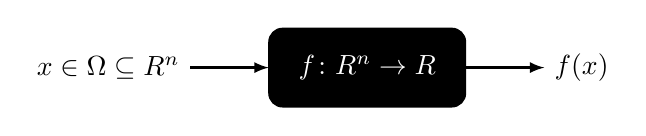
\begin{tikzpicture}
                \draw[-latex,thick] (0,0) node[left] {$x \in \Omega \subseteq \R^n$} -- (1,0);
                \draw[rounded corners=5pt,fill=black] (1,-.5) rectangle (3.5,.5);
                \node[color=white] at (2.25,0) {$f \colon \R^n \to \R$};
                \draw[-latex,thick] (3.5,0) -- (4.5,0) node[right] {$f(x)$};
            \end{tikzpicture}
        \end{figure}
        \item $f$ may be smooth, but~$\nabla f$ \alert{cannot be numerically evaluated}.
        \item Evaluations of~$f$ can be \alert{noisy} and \alert{expensive}.
        \begin{figure}
            \medskip
            \centering
            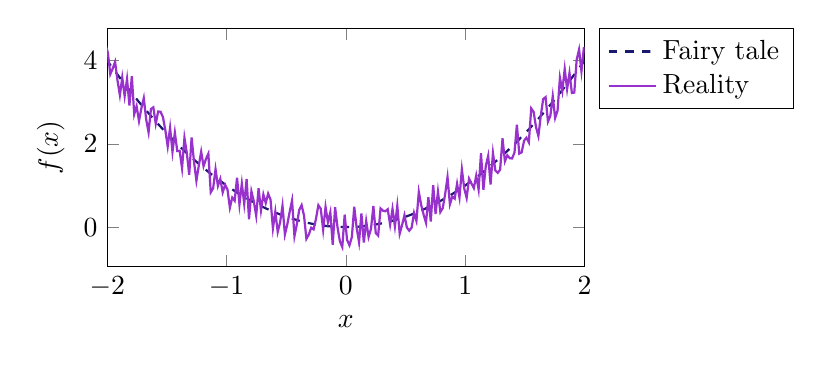
\begin{tikzpicture}
                \begin{axis}[scale only axis=true,width=.5\textwidth,height=.25\textwidth,legend pos=outer north east,legend cell align=left,xmin=-2,xmax=2,xlabel={$x$},ylabel={$f(x)$}]
                    \addplot[no markers,thick,dashed,MidnightBlue,smooth,samples=50] {x*x};
                    \addplot[no markers,thick,DarkOrchid,samples=500] {x*x+.5*rand};
                    \legend{Fairy tale,Reality}
                \end{axis}
            \end{tikzpicture}
        \end{figure}
    \end{itemize}
\end{frame}

\begin{frame}
    \frametitle{An example of \gls{dfo} problem}

    \begin{figure}
        \centering
        \begin{tikzpicture}[scale=.9, every node/.style={transform shape}]
            \uncover<2>{\draw[pattern=north west lines,pattern color=mLightBrown!40,rounded corners=5pt] (8,3) rectangle (11,4.5);}
            \draw[thick,rounded corners=5pt] (0,0) rectangle (3,1.5);
            \draw[thick,rounded corners=5pt] (0,4) rectangle (3,5.5);
            \draw[thick,rounded corners=5pt] (4,2) rectangle (7,3.5);
            \draw[thick,rounded corners=5pt] (8,1) rectangle (11,2.5);
            \only<1>{\draw[thick,rounded corners=5pt] (8,3) rectangle (11,4.5);}
            \uncover<2>{\draw[thick,rounded corners=5pt,color=mLightBrown] (8,3) rectangle (11,4.5);}
            \draw[thick,-latex] (3,1) -- (5.5,1) -- (5.5,2);
            \draw[thick] (3,0.5) -- (7.5,0.5) -- (7.5,2.5) -- (7,2.5);
            \draw[thick,-latex] (7.5,1.75) -- (8,1.75);
            \draw[thick] (3,4.75) -- (7.5,4.75) -- (7.5,3) -- (7,3);
            \draw[thick,-latex] (7.5,3.75) -- (8,3.75);
            \node at (0.6,0.75) {
\includegraphics[height=0.8cm]{ml/presentation.png}};
            \node at (0.6,4.75) {
\includegraphics[height=0.8cm]{ml/checklist.png}};
            \node at (4.6,2.75) {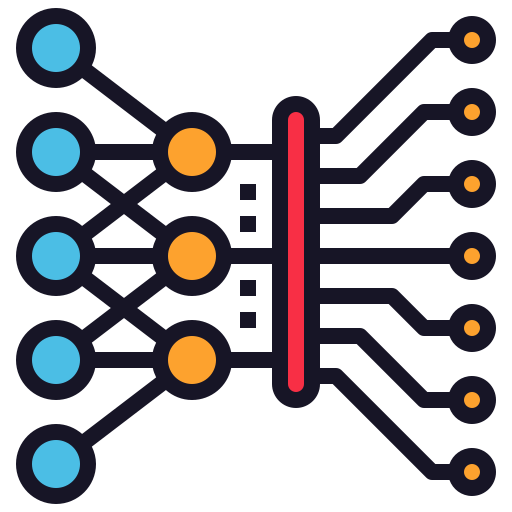
\includegraphics[height=0.8cm]{ml/deep-learning.png}};
            \node at (8.6,1.75) {
\includegraphics[height=0.8cm]{ml/good.png}};
            \node at (8.6,3.75) {
\includegraphics[height=0.8cm]{ml/result.png}};
            \node at (2,0.75) {\makecell{Training\\ dataset}};
            \node at (2,4.75) {\makecell{Testing\\ dataset}};
            \node at (6,2.75) {\makecell{Machine\\ Learning\\ model}};
            \node at (10,1.75) {\makecell{Training\\ accuracy}};
            \node at (10,3.75) {\makecell{Testing\\ accuracy}};
            \uncover<2>{
                \draw[pattern=north west lines,pattern color=mLightBrown!40,rounded corners=5pt] (0,2) rectangle (3,3.5);
                \draw[thick,color=mLightBrown,rounded corners=5pt] (0,2) rectangle (3,3.5);
                \draw[thick,-latex] (3,2.75) -- (4,2.75);
                \node at (0.6,2.75) {
\includegraphics[height=0.8cm]{ml/technical-support.png}};
                \node at (2,2.75) {\makecell{Hyper-\\params}};
            }
        \end{tikzpicture}
    \end{figure}

    \uncover<2>{How to \alert{optimize} the accuracy of the model by tuning the \alert{hyperparameters}? What is the gradient of the performance of the model (e.g., testing accuracy) with respect to the hyperparameters?}
\end{frame}

\section{Powell's derivative-free solvers}

\begin{frame}
    \frametitle{Two paradigms of methods}

    \begin{itemize}
        \setlength{\itemsep}{\bigskipamount}
        \item \alert{Direct-search methods}: sampling iteratively~$f$ at a finite number of points and choosing the iterates using simple comparisons.
        \begin{itemize}
            \item \textit{Examples}: Nelder-Mead, GPS, MADS, BFO, \dots
        \end{itemize}
        \item \alert{Model-based methods}: modeling iteratively~$f$ using simple functions and choosing the iterates by minimizing the models.
        \begin{itemize}
            \item \textit{Globalization}: embedded in \alert{trust-region} or line-search frameworks.
            \item \textit{Examples}: Powell's solvers, DFO, ORBIT, BOOSTERS, DFO-LS, \dots
        \end{itemize}
    \end{itemize}

    \begin{exampleblock}{Idea of trust-region frameworks}
        Given a model~$f_k$ of~$f$ around~$x_k$, the trial step~$d_k$ approximates
        $$\argmin \set[\big]{f_k(x_k + d) : x_k + d \in \Omega_k, \norm{d} \le \Delta_k },$$
        where~$\Delta_k$ is the trust-region radius and~$\Omega_k \approx \Omega$ around~$x_k$.
        Accept the trial point~$x_k + d_k$ if it satisfies some \alert{reduction condition}, and update the trust-region radius~$\Delta_k$ accordingly.
    \end{exampleblock}
\end{frame}

\begin{frame}
    \frametitle{General overview of the Powell's derivative-free solvers}

    Powell developed five \alert{derivative-free trust-region} solvers.

    \begin{minipage}{\textwidth}
        \setcounter{mpfootnote}{\value{footnote}}
        \renewcommand{\thempfootnote}{\arabic{mpfootnote}}
        \begin{table}
            \centering
            \begin{tabular}{@{}llll@{}}
                \toprule
                \textbf{Solvers}    & \textbf{References}       & \textbf{Constraint types} & \textbf{Model types}\\
                \midrule
                \gls{cobyla}        & \textcite{Powell_1994}    & nonlinear                 & linear (FD\footnote{FD: obtained by fully-determined interpolations.})\\
                \gls{uobyqa}        & \textcite{Powell_2002}    & unconstrained             & quadratic (FD)\\
                \gls{newuoa}        & \textcite{Powell_2006}    & unconstrained             & quadratic (UD\footnote{UD: obtained by underdetermined interpolations.})\\
                \gls{bobyqa}        & \textcite{Powell_2009}    & bounds                    & quadratic (UD)\\
                \gls{lincoa}        & \textcite{Powell_2015}    & linear                    & quadratic (UD)\\
                \bottomrule
            \end{tabular}
        \end{table}
        \setcounter{footnote}{\value{mpfootnote}}
    \end{minipage}

    \begin{exampleblock}{Original implementation of the solvers}
        Powell implemented the five solvers in \alert{Fortran 77} \dots
    \end{exampleblock}
\end{frame}

\begin{frame}
    \frametitle{Models for \gls{newuoa}, \gls{bobyqa}, and \gls{lincoa}}

    Given a nondegenerate \alert{interpolation set}~$\mathcal{X}_k \subseteq \R^n$, the~$k$th \alert{quadratic model}~$f_k$ of the objective function~$f$ solves
    \begin{align*}
        \min        & \quad \norm[\big]{\nabla^2 Q - \nabla^2 f_{k - 1}}_{\mathsf{F}}\\
        \text{s.t.} & \quad Q(x) = f(x), ~ x \in \mathcal{X}_k,\\
                    & \quad Q \in \mathcal{Q}_n,
    \end{align*}
    where~$\mathcal{Q}_n$ is the set of quadratic functions in~$\R^n$.

    \begin{itemize}
        \item Typically,~$\mathcal{X}_k$ has~\alert{$\mathcal{O}(n)$} elements, instead of~$\mathcal{O}(n^2)$.
        \item At each iteration, at most one point of~$\mathcal{X}_k$ is modified, causing an at-most \alert{rank-$2$ update} of the KKT matrix of the system.
        \item Geometry of~$\mathcal{X}_k$ is maintained using \alert{Lagrange polynomials}.
    \end{itemize}
\end{frame}

\section{The \glsfmttext{pdfo} package}

\begin{frame}
    \frametitle{Current version of the \gls{pdfo} package}

    \begin{exampleblock}{Interfaces for Powell's solvers}
        PDFO provides MATLAB/Python \alert{interfaces} for using Powell's derivative-free solvers.
        \addtolength{\leftmargini}{\dimexpr\medskipamount+.2ex\relax}
        \begin{itemize}
            \item More \alert{languages} will be added in the future.
            \item It supports Linux, MacOS, and \alert{even Windows}.
            \item It is \alert{NOT} a reimplementation, but rather interfaces (reimplementation will come in the future)!
        \end{itemize}
    \end{exampleblock}

    \begin{figure}
        \centering
        \begin{tikzpicture}
            \node at (0,0) {
\includegraphics[width=6em]{pdfo.png}};
            \node [right] at (1.5,0.25) {Visit \gls{pdfo} homepage};
            \node [right] at (1.5,-0.25) {\usebeamercolor[fg]{structure}\url{https://www.pdfo.net/}};
        \end{tikzpicture}
    \end{figure}
\end{frame}

\begin{frame}
    \frametitle{Current version of the \gls{pdfo} package}

    \begin{figure}
        \centering
        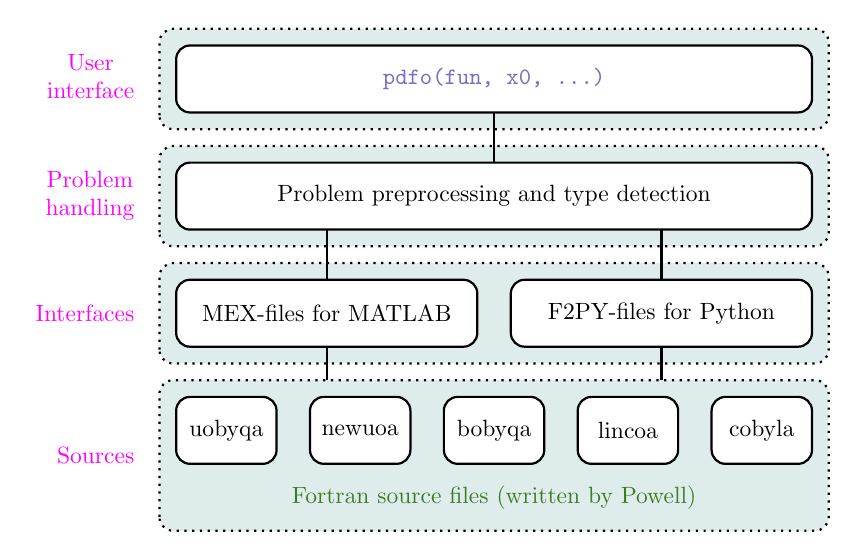
\begin{tikzpicture}[scale=.85, every node/.style={transform shape}]
            \draw[thick,dotted,rounded corners=5pt,fill=CadetBlue!20] (-.25,-1) rectangle (9.75,1.25);
            \draw[thick,rounded corners=5pt,fill=white] (0,0) rectangle (1.5,1);
            \draw[thick,rounded corners=5pt,fill=white] (2,0) rectangle (3.5,1);
            \draw[thick,rounded corners=5pt,fill=white] (4,0) rectangle (5.5,1);
            \draw[thick,rounded corners=5pt,fill=white] (6,0) rectangle (7.5,1);
            \draw[thick,rounded corners=5pt,fill=white] (8,0) rectangle (9.5,1);
            \node at (0.75,0.5) {\gls{uobyqa}};
            \node at (2.75,0.5) {\gls{newuoa}};
            \node at (4.75,0.5) {\gls{bobyqa}};
            \node at (6.75,0.5) {\gls{lincoa}};
            \node at (8.75,0.5) {\gls{cobyla}};
            \node at (4.75,-.5) {\textcolor{OliveGreen}{Fortran source files (written by Powell)}};
            \node[left] at (-.5,0.125) {\textcolor{Fuchsia}{Sources}};
            \draw[thick,dotted,rounded corners=5pt,fill=CadetBlue!20] (-.25,1.5) rectangle (9.75,3);
            \draw[thick,rounded corners=5pt,fill=white] (0,1.75) rectangle (4.5,2.75);
            \draw[thick,rounded corners=5pt,fill=white] (5,1.75) rectangle (9.5,2.75);
            \node at (2.25,2.25) {MEX-files for MATLAB};
            \node at (7.25,2.25) {F2PY-files for Python};
            \node[left] at (-0.5,2.25) {\textcolor{Fuchsia}{Interfaces}};
            \draw[thick,dotted,rounded corners=5pt,fill=CadetBlue!20] (-.25,3.25) rectangle (9.75,4.75);
            \draw[thick,rounded corners=5pt,fill=white] (0,3.5) rectangle (9.5,4.5);
            \node at (4.75,4) {Problem preprocessing and type detection};
            \node[left] at (-0.5,4) {\textcolor{Fuchsia}{\makecell{Problem\\ handling}}};
            \draw[thick,dotted,rounded corners=5pt,fill=CadetBlue!20] (-.25,5) rectangle (9.75,6.5);
            \draw[thick,rounded corners=5pt,fill=white] (0,5.25) rectangle (9.5,6.25);
            \node at (4.75,5.75) {\textcolor{Periwinkle}{\texttt{pdfo(fun, x0, ...)}}};
            \node[left] at (-0.5,5.75) {\textcolor{Fuchsia}{\makecell{User\\ interface}}};
            \draw[thick] (2.25,1.25) -- (2.25,1.75);
            \draw[thick] (7.25,1.25) -- (7.25,1.75);
            \draw[thick] (2.25,2.75) -- (2.25,3.5);
            \draw[thick] (7.25,2.75) -- (7.25,3.5);
            \draw[thick] (4.75,4.5) -- (4.75,5.25);
        \end{tikzpicture}
    \end{figure}
\end{frame}

\begin{frame}
    \frametitle{Core features of \gls{pdfo}}

    \begin{exampleblock}{\gls{pdfo} preprocesses a problem as follows}
        \addtolength{\leftmargini}{\dimexpr\medskipamount+.2ex\relax}
        \begin{itemize}
            \item Detect obvious \alert{infeasibility}.
            \item Attempt to \alert{project the initial guess} onto the feasible set for linearly-constrained problems.
            \item Eliminate \alert{linear equality constraints} (QR factorization).
            \item \alert{Reformulate the constraints} to call the Powell's solvers.
            \item Handle possible \alert{overflows} and \alert{faults} of the inputs.
        \end{itemize}
    \end{exampleblock}

    Minor modifications to the Fortran source code have been made.
    \begin{itemize}
        \item The original \gls{cobyla} code may \alert{NOT return} the best evaluated point.
        \item The original \gls{uobyqa} and \gls{lincoa} code might encounter \alert{infinite cyclings} on \textcolor{BrickRed}{ill-conditioned problems}.
        \item Other programming-related bugs have also been patched.
    \end{itemize}
\end{frame}

\begin{frame}
    \frametitle{Comparison of the Powell's solvers using \gls{pdfo}}

    We tested \alert{\gls{pdfo}} using performance profiles\footnote{See~\textcite{Dolan_More_2002, More_Wild_2009}.} on problems from the CUTEst\footnote{We used the PyCUTEst package by J. Fowkes and L. Roberts.} dataset of \textcite{Gould_Orban_Toint_2015}.

    \begin{figure}
        \centering
        \only<1>{%
            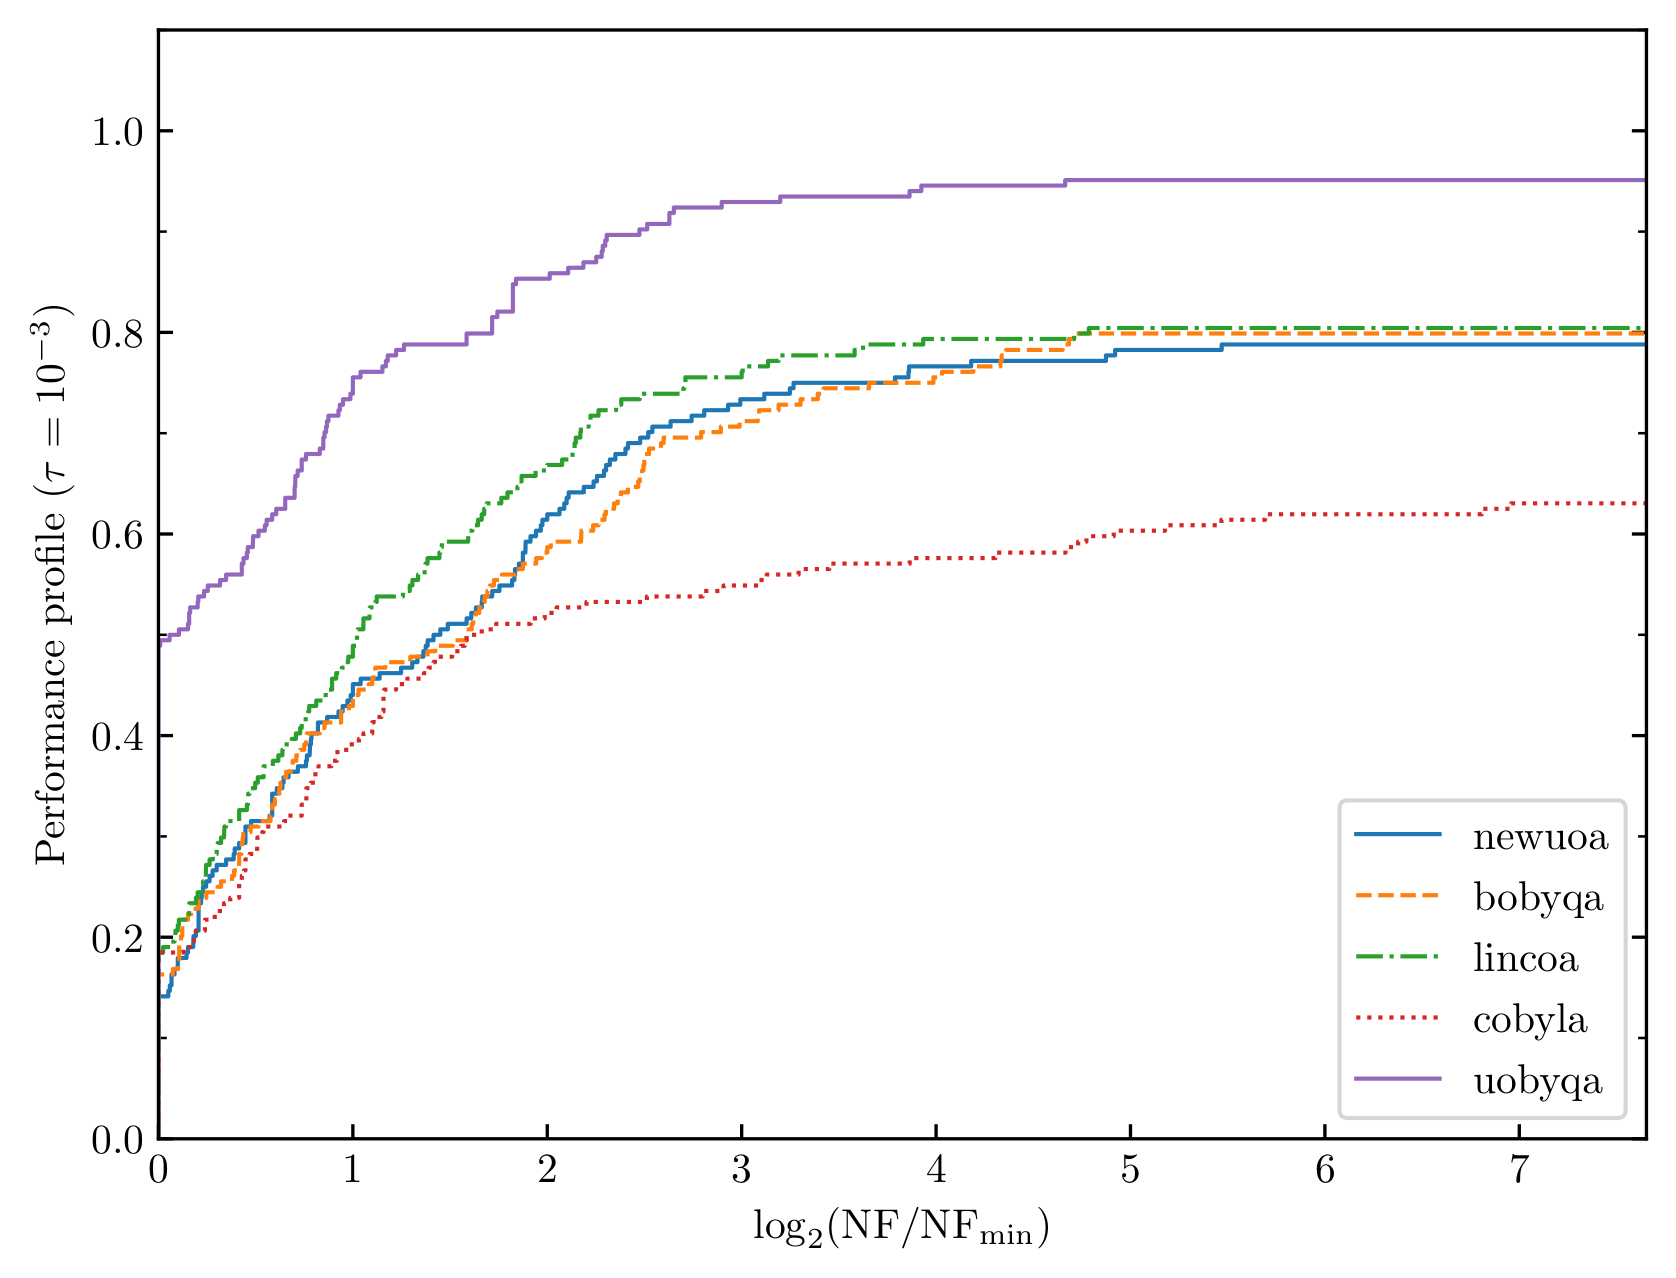
\includegraphics[height=.4\textwidth]{cutest_10.png}
            \caption{\alert{Unconstrained} problems of dimensions \alert{at most~$10$}}
        }
        \only<2>{%
            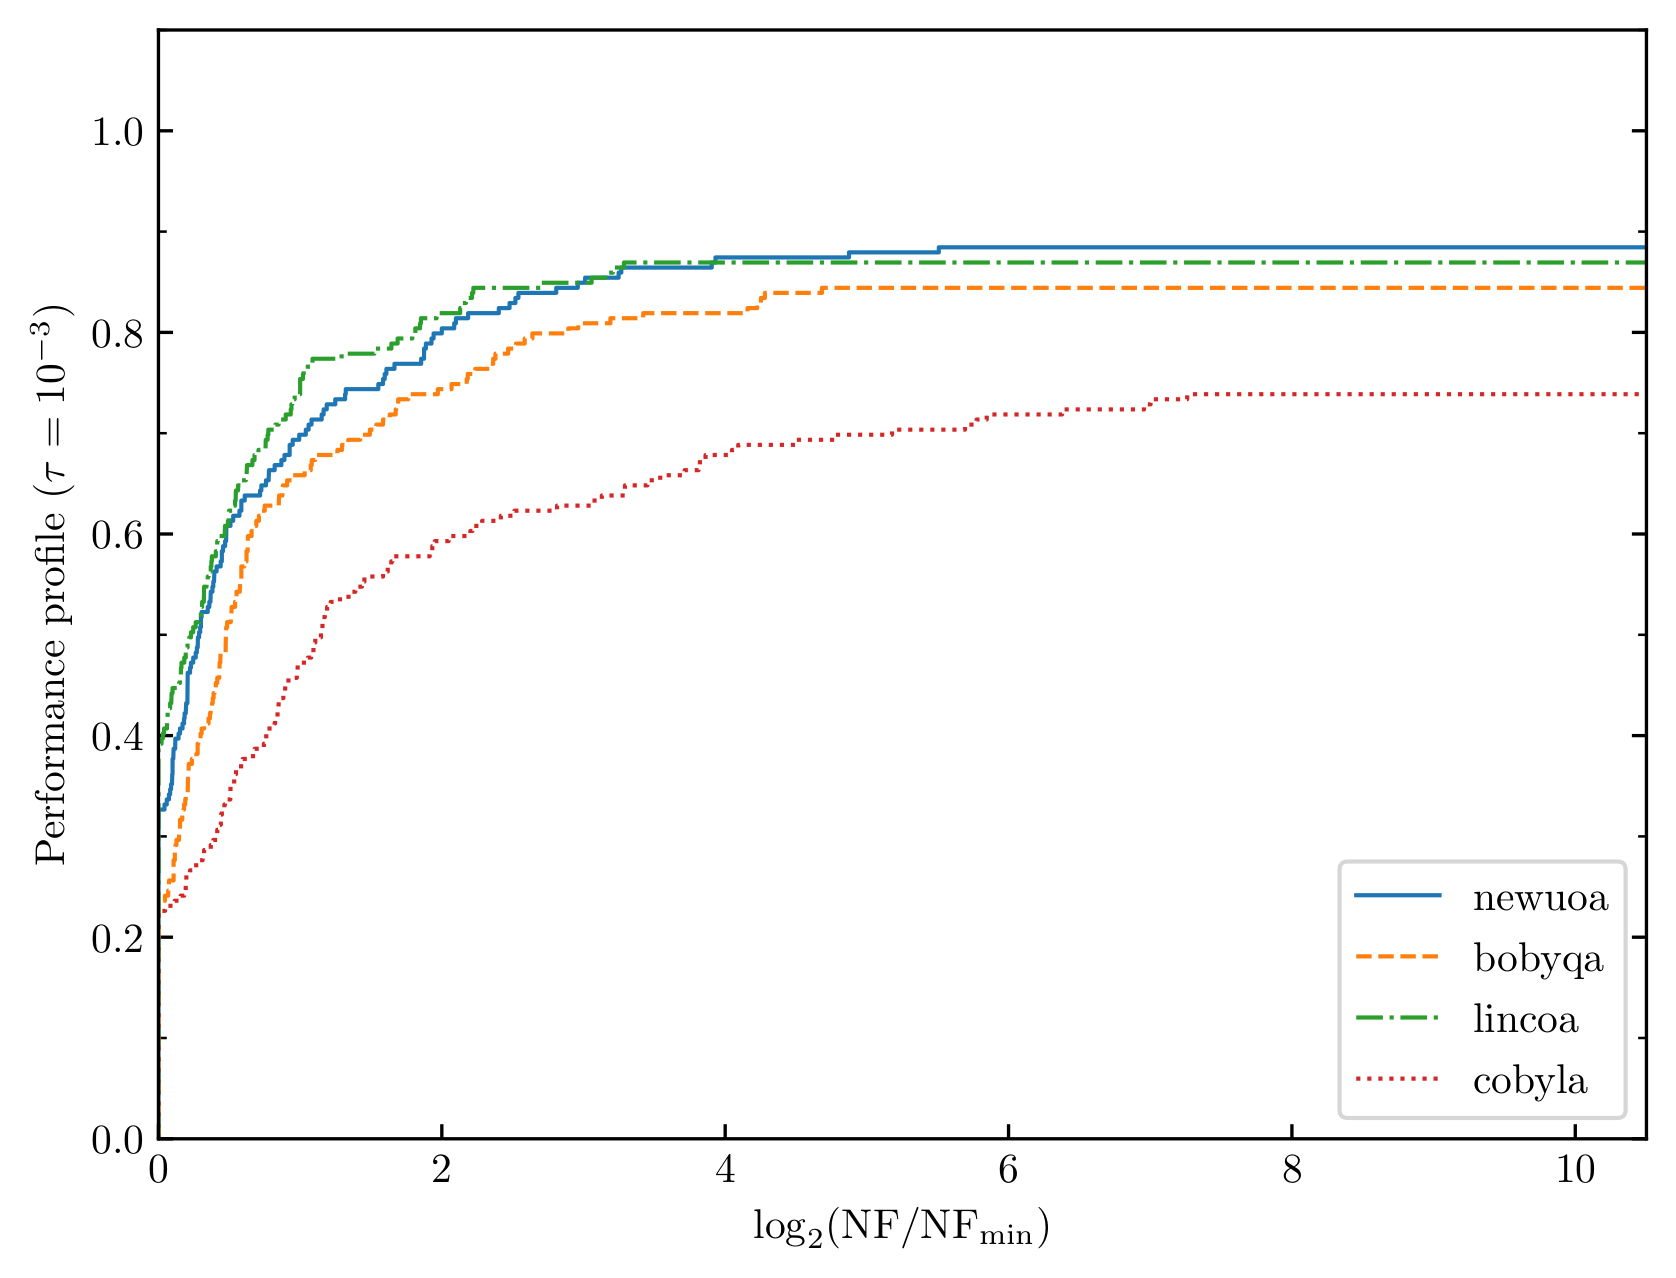
\includegraphics[height=.4\textwidth]{cutest_50.png}
            \caption{\alert{Unconstrained} problems of dimensions \alert{at most~$50$}}
        }
        \only<3>{%
            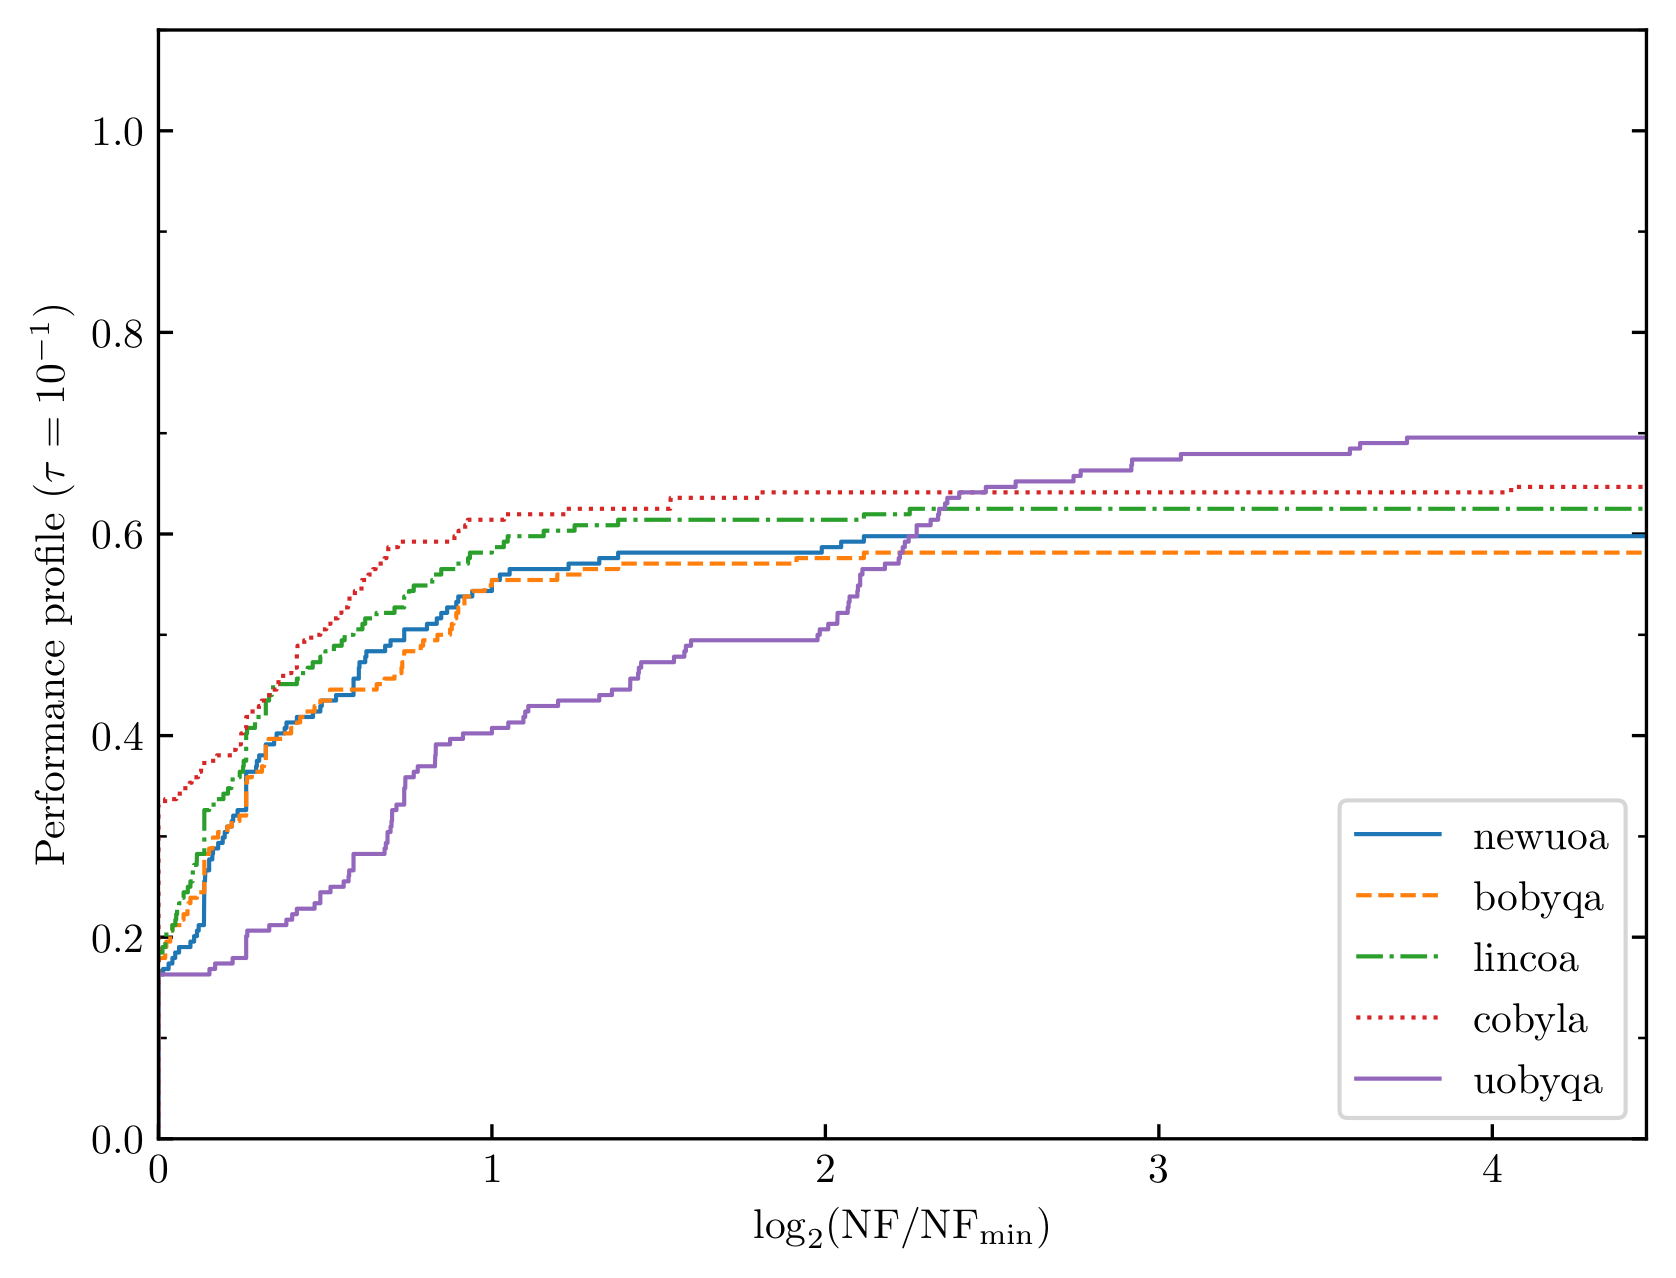
\includegraphics[height=.4\textwidth]{cutest_10_noisy.png}
            \caption{\alert{Unconstrained noisy} problems of dimensions \alert{at most~$10$}}
            % Noise level is 1e-2
        }
    \end{figure}
\end{frame}

\begin{frame}[c,allowframebreaks]
    \frametitle{A synthetic noisy nonsmooth problem}

    Consider the \alert{noisy Rosenbrock-like nonsmooth} function
    $$f(x) = \big(1 + \sigma e(x)\big) r(x) \quad \text{with} \quad r(x) = \sum_{i = 1}^{n - 1} 4 \abs[\big]{x_{i + 1} - x_i^2} + \abs{1 - x_i},$$
    where~$e(x) \sim \mathcal{N}(0, 1)$ and~$\sigma \ge 0$.
    In our experiment:
    \begin{itemize}
        \item dimension is~$n = 10$,
        \item constraints are~$-10 \le x_i \le 1 / i$ for all~$i = 1, 2, \dots, n$,
        \item noise level is~\alert{$\sigma = 0.1$},
        \item budget is~\alert{$100$} function evaluations, and
        \item number of random experiments is~$20$.
    \end{itemize}

    \framebreak

    \begin{figure}
        \centering
        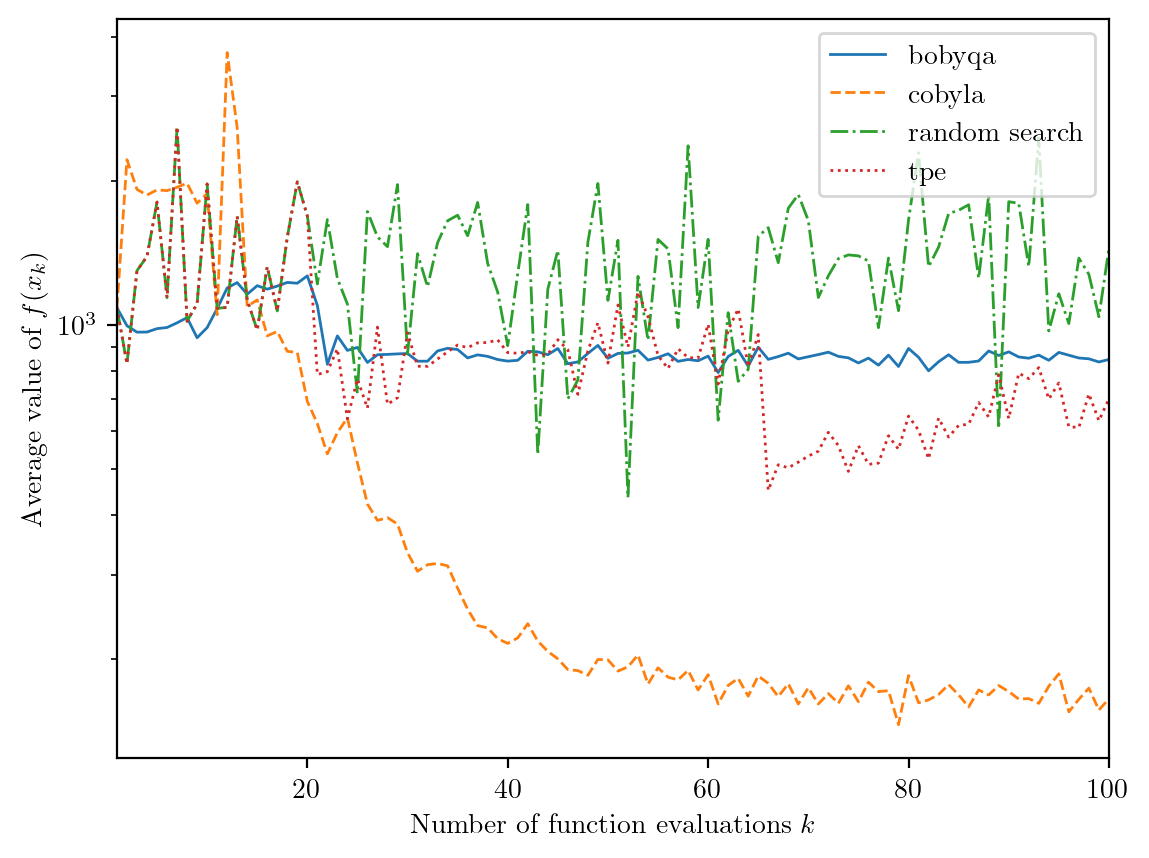
\includegraphics[width=.85\textwidth]{comp.png}
    \end{figure}
\end{frame}

\begin{frame}
    \frametitle{A hyperparameter tuning problem}

    Similarly to~\textcite{Bradley_1997, Ghanbari_Scheinberg_2017}, consider the following \alert{hyperparameter tuning problem}: optimize the \alert{AUC score}\footnote{See \textcite{Hanley_Mcneil_1982}.} of an SVM (2 hyperparameters) in \alert{binary classification} on given LIBSVM\footnote{Available at \url{https://www.csie.ntu.edu.tw/~cjlin/libsvm/}.} datasets.

    \medskip

    \only<1>{
        \begin{table}
            \centering
            \caption{Dataset \enquote{splice} ($1,000$ data,~$60$ features)}
            \begin{tabular}{@{}lccc@{}}
                \toprule
                \multicolumn{1}{c}{Solvers}	& No. evaluations	& AUC Scores	& Testing accuracies\\
                \midrule
                PDFO						& $65$				& $0.96$	    & $0.89$\\
                Random search				& $100$				& $0.64$	    & $0.53$\\
                Random search				& $200$				& $0.79$	    & $0.53$\\
                TPE (Bayesian)				& $100$				& $0.50$	    & $0.50$\\
                \bottomrule
            \end{tabular}
        \end{table}
    }
    \only<2>{
        \begin{table}
            \centering
            \caption{Dataset \enquote{ijcnn1} ($49,990$ data,~$22$ features)}
            \begin{tabular}{@{}lccc@{}}
                \toprule
                \multicolumn{1}{c}{Solvers}	& No. evaluations	& AUC Scores	& Testing accuracies\\
                \midrule
                PDFO						& $59$				& $0.99$	    & $0.98$\\
                Random search				& $100$				& $0.98$	    & $0.97$\\
                Random search				& $200$				& $0.98$	    & $0.97$\\
                TPE (Bayesian)				& $100$				& $0.98$	    & $0.98$\\
                \bottomrule
            \end{tabular}
        \end{table}
    }
\end{frame}

\section{Summary and conclusion}

\begin{frame}
    \frametitle{Summary and conclusion}

    \begin{itemize}
        \setlength{\itemsep}{\bigskipamount}
        \item We have developed an \alert{initial version of \gls{pdfo}}.
        \begin{itemize}
            \item It provides \alert{MATLAB/Python interfaces} for Powell's \gls{dfo} solvers.
            \item \alert{Encouraging feedbacks} are received from both academia and industry (IRT Saint-Exup{\'{e}}ry, Toulouse, France).
            \item We made \alert{brief comparisons} with Bayesian optimization.
        \end{itemize}
        \item We are now working on a \alert{new derivative-free trust-region method} for nonlinear constrained problems, to be included in \gls{pdfo}.
    \end{itemize}

    \begin{minipage}{.29\textwidth}
        \begin{figure}
            \centering
            
\includegraphics[width=6em]{pdfo.png}
        \end{figure}
    \end{minipage}
    \begin{minipage}{.69\textwidth}
        {\huge Thank you!}

        \medskip

        {\small Contact: \alert{\href{mailto:tom.ragonneau@connect.polyu.hk}{\texttt{tom.ragonneau@connect.polyu.hk}}}.}
    \end{minipage}
\end{frame}

\appendix

\begin{frame}[t,allowframebreaks]
    \frametitle{References}

    \printbibliography[heading=none]
\end{frame}

\end{document}